\documentclass[11pt]{scrartcl}
\usepackage{dominatrix}
\usepackage{colortbl}
\usepackage{pgfplots}
\newcommand{\jon}{J\'{o}n }
\newcommand{\oneth}{\ensuremath{\frac{1}{3}}}
\newcommand{\twoth}{\ensuremath{\frac{2}{3}}}
\newcommand{\ve}{\varepsilon}
\pgfplotsset{compat=1.9}
\definecolor{light-gray}{gray}{0.75}
\title{Solow-Swan Growth Model}
\subject{ECON W3213 Spring 2014 \jon Steinsson}
\author{Linan Qiu, lq2137}
\begin{document}

\maketitle

\begin{abstract}
This set of recitation notes covers the \textbf{Solow-Swan Growth Model } This is in no way a substitute for attending lectures, but just in case you dozed off or checked your boyfriend's Facebook page while \jon was working Calculus magic on the board, this set of notes may save you.

Also, do call it the Solow-Swan model, not the Solow model. The model was independently devised by both economists. Independently. Trevor Swan had a part in it too. In fact, he is, I quote Wikipedia, "one of the finest economists not to receive a Nobel prize." Solow got lots of shiny medals already, so I'm sure he'll be fine with Swan tagging along.

Finally, I use the term income and production interchangeably. 
\end{abstract}

\section{Introduction to Growth Models}

In the last set of notes and this one, you will be learning about growth models. Essentially, they answer the question

\begin{quote}
What makes an economy grow?
\end{quote}

And we're not talking about little movements (that economists call "cyclical"). Rather, we're talking about long run trajectories that last tens or even hundreds of years.

Do understand the characteristics of these models. What do I mean? Each model has its inherent assumptions on production and growth. Identify them:

\begin{itemize}
\item What is the key factor of production?
\item What is the production dependent on?
\item What happens in the long run?
\item What happens during shocks both temporary and permanent?
\end{itemize}

This provides a good way for you to contrast the different models and to organize your thoughts. Otherwise, you'd be lost in a sea of information. Not even the CC swim test can help you with that.

One last thing -- we are always talking about real income or real production in these models. We don't factor in inflation at all. In fact, you can think of production in terms of perhaps \textbf{Gatorade} (since \jon loves drinking it so much). We will include monetary effects much later on.

\section{Solow-Swan Model}

The characteristics of the Malthus Model are

\begin{itemize}
\item Capital is the key factor of production
\item Production is dependent on labor (or population) and capital
\item Depending on circumstance, we can tend to a steady state capital in the long run
\item Temporary shocks in capital does nothing to change the steady state. 
\end{itemize}

Let's see how we can arrive at these conclusions.

\subsection{Production Function}

Let's start from first principles. We use capital, labor, and technology to produce things. Let's leave inflation and money out of the picture, so imagine we're producing \jon's favorite drink, Gatorade.

\[ Y = \bar{A}K^{\oneth}L^{\twoth} \]

Convince yourself that this function exhibits

\begin{itemize}
\item Constant returns to scale
\item Diminishing returns to labor
\item Diminishing returns to capital (remember this! This is essential to our conclusion)
\end{itemize}

\textbf{Assume for now that population stays constant.}

On a per person basis, where $L$ is the population, we define

\begin{align*}
y &= \bar{A}\left(\frac{K}{L}\right)^{\oneth} \\
&= \bar{A}k^{\oneth}
\end{align*}

\subsection{Consumption, Savings, and Investment}

You either consume or you save, so

\begin{align*}
C &= (1-s)Y \\
c &= (1-s)y
\end{align*}

The second equation is simply in per capita terms. 

What you save becomes investment (because the banks subsequently lend your money to people who use them to start businesses!)

\begin{align*}
I &= sY \\
i &= sy 
\end{align*}

\subsection{Investment and Depreciation}

Now we know that capital stock $K$ changes over time. We invest in new capital, and old ones get broken and useless. It's the circle of life! There's inflow $I$, and outflow $dK$ due to depreciation. Hence,

\begin{align*}
K_{t+1} - K_t &= I - dK_t \\
&= s\bar{A}K^{\oneth}L^{\twoth} - dK_t
\end{align*}

At the steady state, where $K$ doesn't grow, hence $K_{t+1} = K_t$, 

\begin{align*}
s\bar{A}K^{\oneth}L^{\twoth} &= dK_t \\
K_t^{\twoth} &= \frac{s\bar{A}L^{\twoth}}{d} \\
K_t &= \left(\frac{s\bar{A}}{d}\right)^{\frac{3}{2}}L
\end{align*}

\subsection{Putting It All Together}

We can plot this in a graph.

\begin{figure}[ht!]
\centering
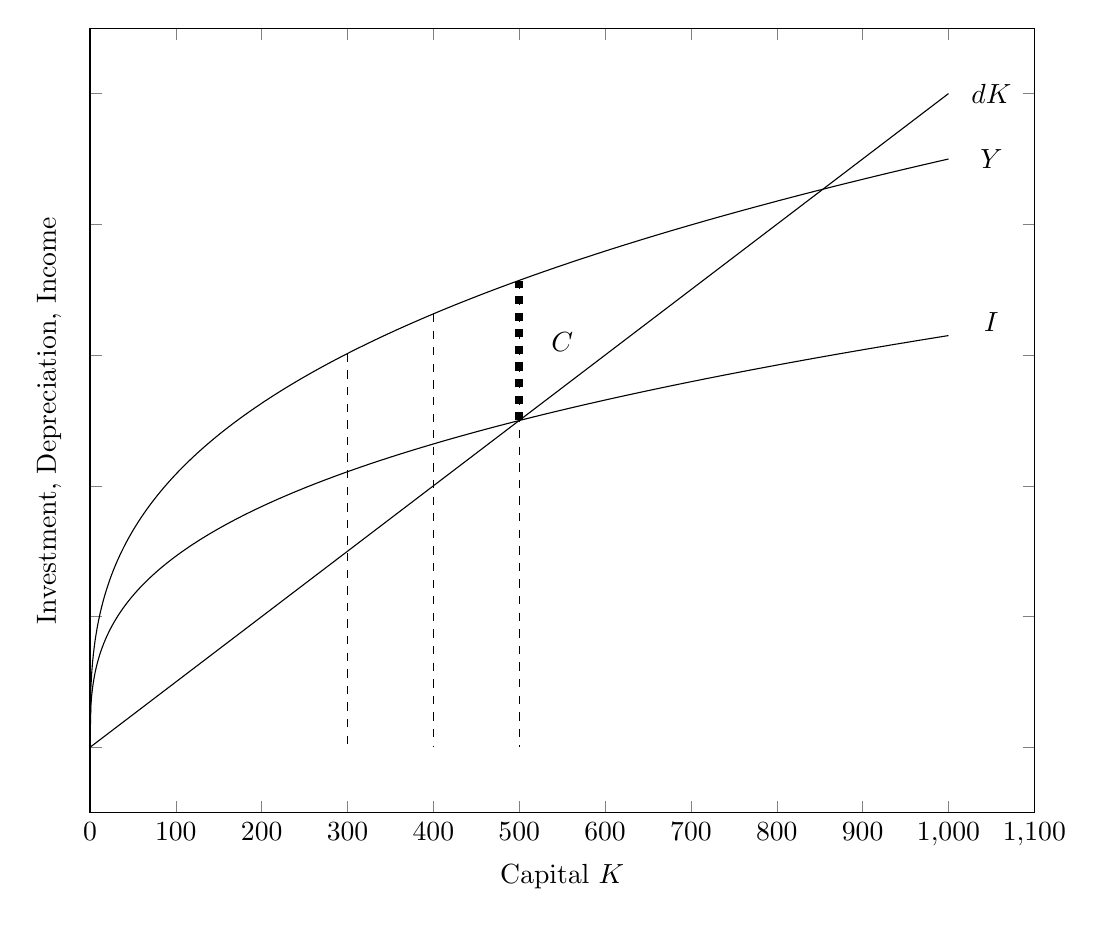
\begin{tikzpicture}
\begin{axis}[ylabel = {Investment, Depreciation, Income}, xlabel={Capital $K$}, yticklabels={,,},scale=1.75, xmin=0]
\addplot[domain=0:1000,black]
{x} node at (axis cs: 1050,1000) {$dK$};
\addplot[domain=0:1000,black,samples=1000]
{62.99*x^(1/3)} node at (axis cs: 1050,650) {$I$};
\addplot[domain=0:1000,black,samples=1000]
{90*x^(1/3)} node at (axis cs: 1050,900) {$Y$};
\addplot[domain=0:1000,black,dashed]
coordinates{(500,714) (500,0)};
\addplot[domain=0:1000,black,dashed]
coordinates{(400,663) (400,0)};
\addplot[domain=0:1000,black,dashed]
coordinates{(300,602) (300,0)};
\addplot[domain=0:1000,black,dashed,line width=3]
coordinates{(500,500) (500,714)} node at (axis cs: 550,620) {$C$};
\end{axis}
\end{tikzpicture}
\caption{Plot of investment, depreciation and income with capital $K$}
\end{figure}

Let's say that originally, we are at $K = 300$. That's below steady state, and we'll move gradually towards the steady state. With a capital injection of $100$, we arrive at $K = 400$. That is still below the steady state, and there is no change to technology nor labor nor savings nor depreciation, so the steady state remains the same, and we're still well on our way to the original steady state at $K=500$. 

When we were at $K=300$, consumption is

\[C_{300} = (1-s)\bar{A}(300)^{\oneth}L^\twoth\]

Graphically, consumption is the vertical distance between Income $Y$ and Investment $I$, because $C = Y-I$. 

a capital injection of $100$ will change consumption by

\[C_{400} = (1-s)\bar{A}(400)^{\oneth}L^\twoth\]

The proportion change is

\[\frac{C_{400}}{C_{300}} = \left(\frac{4}{3}\right)^\oneth\]

However, is there any change in the long run? Nope. Again, we are simply skipping ahead a little, but towards the same steady state $K=500$. Consequently, consumption per capita doesn't change in the long run.

Again, this is because the exogenous factors, savings rate $s$, depreciation $d$, technology $A$.

We can also do this whole exercise in per capita term. We simply have to use per capita equations for investment $i$ and depreciation $dk$

\[ y = \bar{A}\left(\frac{K}{L}\right)^\oneth = \bar{A}k^\oneth \]

\[ i = sy = s\bar{A}\left(\frac{K}{L}\right)^\oneth = s\bar{A}k^\oneth\]

\[ dk = d \frac{K}{L} \]

You can eyeball and see that the graph will still retain the exact same shape.

\subsection{Shocks}

Again, we differentiate between two types of shocks

\begin{itemize}
\item Shocks to capital (sudden changes in capital. For example, in wars.)
\item Shocks to exogenous variables
\end{itemize}

\subsubsection{Shocks to Capital}

Let's say the country we're analyzing is currently at $K = 400$. Suddenly it experienced a war, and capital stock decreased suddenly. Assume also that somehow, no one died (perhaps due to awesome bomb shelters) and all of technology survived. Its capital stock fell to $K=300$. 

\begin{figure}[ht!]
\centering
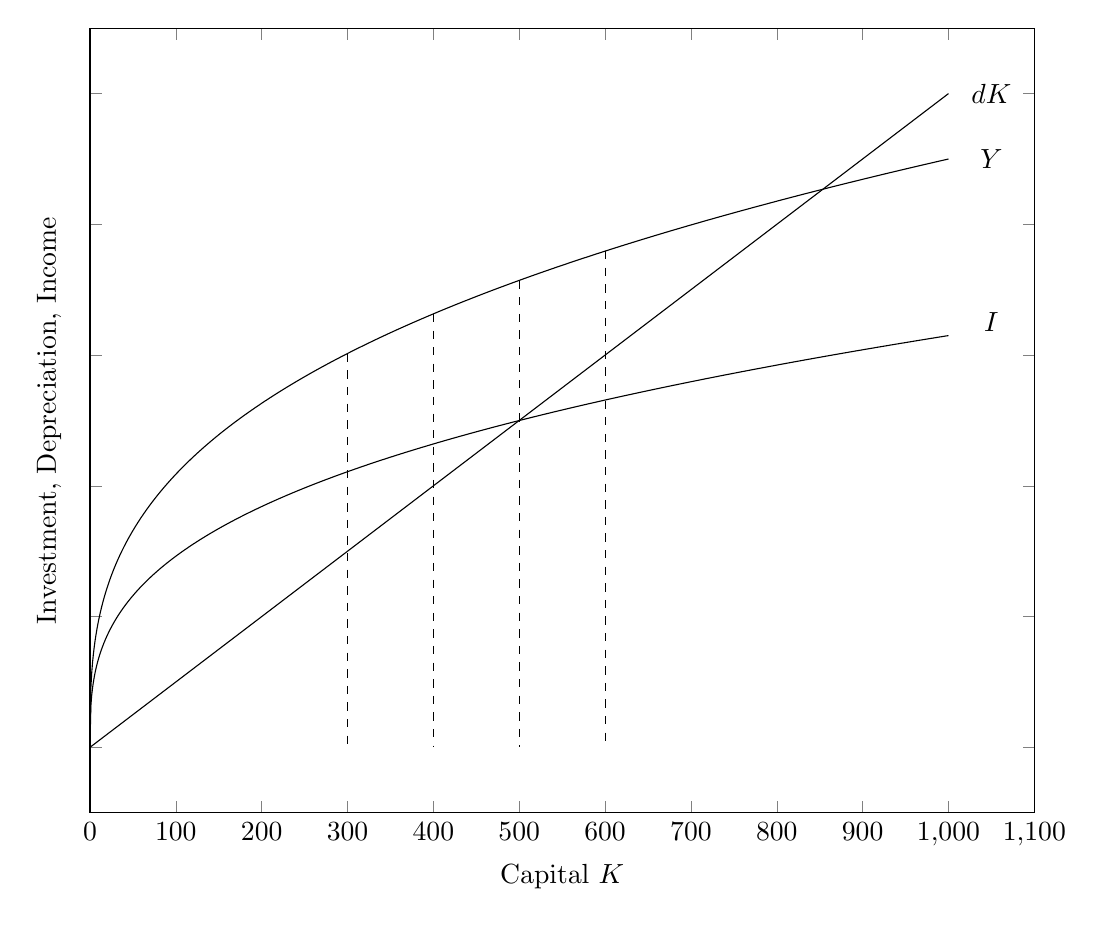
\begin{tikzpicture}
\begin{axis}[ylabel = {Investment, Depreciation, Income}, xlabel={Capital $K$}, yticklabels={,,},scale=1.75, xmin=0]
\addplot[domain=0:1000,black]
{x} node at (axis cs: 1050,1000) {$dK$};
\addplot[domain=0:1000,black,samples=1000]
{62.99*x^(1/3)} node at (axis cs: 1050,650) {$I$};
\addplot[domain=0:1000,black,samples=1000]
{90*x^(1/3)} node at (axis cs: 1050,900) {$Y$};
\addplot[domain=0:1000,black,dashed]
coordinates{(500,714) (500,0)};
\addplot[domain=0:1000,black,dashed]
coordinates{(400,663) (400,0)};
\addplot[domain=0:1000,black,dashed]
coordinates{(300,602) (300,0)};
\addplot[domain=0:1000,black,dashed]
coordinates{(600,759) (600,0)};
\end{axis}
\end{tikzpicture}
\caption{Plot of investment, depreciation and income with capital $K$}
\end{figure}

What will happen in the end? Well, it will simply grow back slowly to steady state capital $\bar{K}$. 

Now if the United Nations pitied us and gave us a capital injection of 300, pushing us to $K=600$. What happens then? Well, we slowly go \textbf{back} to $K=500$, the steady state capital.

In effect, this is saying that without the proper infrastructure and expertise ($\bar{A}$) to handle the additional capital, they will be wasted.

\subsubsection{Shocks to Exogenous Variables}

Now assume that we were originally at $K = 500$, the steady state. Then, technology increased because we discovered penicillin. We can say that

\[A_1 = cA_0\] 

where $c$ is a constant greater than 1 that shows we've grown in terms of technology.

Then,

\[Y_t = cA_0K_t^\oneth L_t^\twoth \]

\[I_t = csA_0K_t^\oneth L_t^\twoth\]

\[C_t =  c(1-s)A_0K_t^\oneth L_t^\twoth\]

\[dK_t = dK_t\] 

Depreciation simply stays the same. 

We find that we arrive at a new steady state

\[\bar{K_0} = c^{\frac{3}{2}}\left(\frac{s\bar{A}}{d}\right)^{\frac{3}{2}}L \]

\begin{figure}[ht!]
\centering
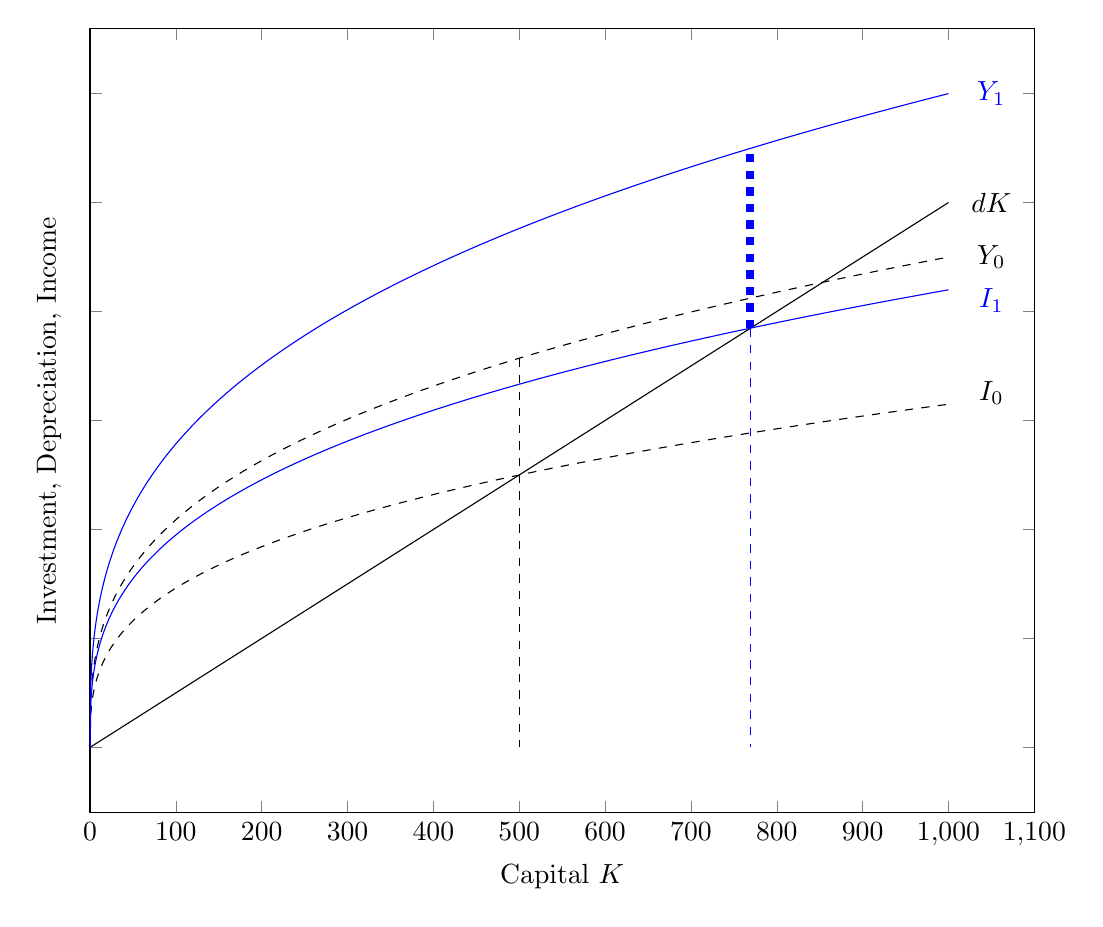
\begin{tikzpicture}
\begin{axis}[ylabel = {Investment, Depreciation, Income}, xlabel={Capital $K$}, yticklabels={,,},scale=1.75, xmin=0]
\addplot[domain=0:1000,black]
{x} node at (axis cs: 1050,1000) {$dK$};
\addplot[domain=0:1000,black,samples=1000, dashed]
{62.99*x^(1/3)} node at (axis cs: 1050,650) {$I_0$};
\addplot[domain=0:1000,black,samples=1000, dashed]
{90*x^(1/3)} node at (axis cs: 1050,900) {$Y_0$};

\addplot[domain=0:1000,black,samples=1000, blue]
{(62.99/90)*120*x^(1/3)} node at (axis cs: 1050,820) {$I_1$};
\addplot[domain=0:1000,black,samples=1000, blue]
{120*x^(1/3)} node at (axis cs: 1050,1200) {$Y_1$};

\addplot[domain=0:1000,black,dashed]
coordinates{(500,714) (500,0)};

\addplot[domain=0:1000,blue,dashed]
coordinates{(769,769) (769,0)};

\addplot[domain=0:1000,blue,dashed,line width=3]
coordinates{(769,769) (769,1100)};

\end{axis}
\end{tikzpicture}
\caption{Plot of investment, depreciation and income with capital $K$}
\end{figure}

Just as what we'd expect, we find that

\begin{itemize}
\item We have a completely new income function
\item We have a completely new investment function
\item Depreciation function stays the same
\item Steady state capital is larger
\item Steady state consumption is larger
\end{itemize}

What happens is that at the original steady state $K=500$, we find that it is no longer a steady state with the new investment function. In fact, there will be positive net investment as investment is larger than depreciation. We will have positive capital growth, and we will keep experiencing that until we arrive at the new steady state.

Try working out the case where \textbf{depreciation changes}

\section{Solow-Swan with Labor Changes}

\subsection{Labor / Population Growth}

For now we've been assuming that labor is constant. Let's try adding in labor changes.

\[L_{t+1} = (1+\bar{n}) L_t \]

Where $\bar{n}$ represents population growth. For example, if population grows by 20\% from period 0 to period 1, then $\bar{n} = 0.2$, hence $L_1 = (1.2)L_0$

\subsection{Production Function}

This is going to confuse our production function, since we have terms all in $t$ terms, and not $t+1$ or $t-1$

\[Y_t = \bar{A}K^\oneth L^\twoth \]

So what we can do is to divide everything throughout by $L_t$. Then,

\[y_t = \bar{A}k^\oneth \]

\[i_t = s\bar{A}k^\oneth \]

\subsection{Steady State Capital and Income}

Let's go back to the capital accumulation equation

\[K_{t+1} - K_t = sY_t - dK_t \]

We can divide this throughout by $L_t$ too

\begin{align*}
\frac{K_{t+1}}{L_t} - \frac{K_t}{L_t} &= s\frac{Y_t}{L_t} - d\frac{K_t}{L_t} \\
\frac{K_{t+1}}{L_t} - k_t &= sy_t - dk_t \\
\frac{K_{t+1}}{\left(\frac{L_{t+1}}{1+\bar{n}}\right)} - k_t &= sy_t - dk_t \\
k_{t+1} (1+\bar{n}) - k_t &= sy_t - dk_t
\end{align*}

In the third equation, we're using the fact that

\begin{align*}
L_{t+1} &= (1+\bar{n})L_t \\
L_t &= \frac{L_{t+1}}{1+\bar{n}}
\end{align*}

Now the steady state capital equation is kind of ugly, so let's make it prettier so that we can draw graphs. Think about it. You can't draw graphs of $k_{t+1}$ against $k_t$ if you have the fugly $(1+\bar{n})$ inside there right?

\begin{align*}
k_{t+1} (1+\bar{n}) - k_t &= sy_t - dk_t \\
k_{t+1} - k_t &= \frac{1}{1+\bar{n}}\left[sy_t - (d + \bar{n})k_t\right]
\end{align*}

Now we don't even need to plot this to know that we will get a steady state, and the graph is going to pretty much look the same. Depreciation line is going to have its gradient increased by $\bar{n}$, and they're both going to be scaled by $\frac{1}{1+\bar{n}}$. 

We can also solve for steady state $\bar{k}$.

\[\bar{k} = \left(\frac{s\bar{A}}{d+\bar{n}}\right)^\frac{3}{2} \]

The corresponding steady state income is going to be 

\[\bar{y} = \left(\frac{s}{d+\bar{n}}\right)^\frac{1}{2} \bar{A}^\frac{3}{2}\]

Intuitively, this is what's happening. Depreciation line changed because we're measuring capital on a \textbf{per capita} basis. Then, if population grows, we are "diluting" capital to more people, hence it is almost like as if capital per capita is decreasing, hence depreciating at a faster rate. Both the investment inflow and depreciation outflow have smaller effects by $\frac{1}{1+\bar{n}}$ again because we're measuring in per capita terms, and population growth causes a kind of "dilution."

Now if per capita output, capital and consumption is constant, the growth rate of the \textbf{level of output, capital and consumption} will be at $\bar{n}$, since the only growth at steady state \textbf{per capita} capital comes from labor.

%\section{Solow-Swan with Technology Changes}
%
%\subsection{Technology Growth}
%
%Since we're throwing in labor changes, we might as well throw in technology changes as well. 
%
%\[ A_{t+1} = A_t(1+\bar{g}) \]
%
%Let's try this using the exact same method as we did -- by dividing everything throughout by $A_tL_t$ (since labor is changing at the same time as well).
%
%\subsection{Steady State Capital and Income (Wrong Method)}
%
%\begin{align*}
%Y_t &= A_tK_t^\oneth L_t^\twoth \\
%\frac{Y_t}{A_tL_t} &= \left(\frac{K_t}{L_t}\right)^\oneth \\
%y_t &= k_t^\oneth
%\end{align*}
%
%This seems kind of familiar right? 
%
%Then we have
%
%\[ k_{t+1} - k_t = \frac{1}{(1+\bar{n})(1+\bar{g})} \left[sy_t - (d-1+(1+\bar{n}) (1+\bar{g}))k_t \right] \]
%
%Solving for steady state, 
%
%\begin{align*}
%s{\bar{k}^\oneth} &= (d-1+(1+\bar{n}) (1+\bar{g}))\bar{k} \\
%\bar{k} &= 
%\end{align*}

\section{Convergence}

Now let's test our model. Let's assume that all countries have the same parameters $\bar{A}$, $d$, $s$. Then in that case, their \textbf{capital per capita} $k$ should all converge to the same amount. 

Is that happening? Well, not really empirically. You can look up the data in \jon's slides, but the idea is that not every country has the same parameters. For example, asian countries tend to have a much higher savings rate than its western counterparts.

Hence \textbf{unconditional convergence} -- the idea that countries' capital per capita and hence economic growth converges no matter what their idiosyncratic conditions are, is \textbf{false}.

\textbf{Conditional convergence} -- the idea that they converge only if they have similar conditions (eg. savings rate, depreciation, and more importantly, technology) is \textbf{empirically supported} to a large extent.

We went on a huge roundabout just to arrive at this commonsensical conclusion. Wow.

\end{document}